\chapter{Dark matter}

\label{ch:dm}

\section{Introduction}
\par As mentioned in the previous chapter, about one quater of the total mass-energe in universe are dark matter.
Up till now, there is no specific particle that can account for all of the Dark Matter in the universe. And it became popular to consider Dark Matter as a whole sector of new particles, instead of the existence of a single new type of particle.\\
This Chapter is organized as follows: section 3.1.1 discusses the origin and evidence of Dark Matter and 
section 3.1.2 introduced the Dark Matter theory. In section 3.2, one candidate of Dark Matter, Weakly Interacting Massive Particles, is described. Finally, Section 3.3 outlines how Dark Matter particles might be produced by particle colliders and what signatures they might have.

\par The concept of dark matter is originated from cosmology observation. A variety of astrophysical observations at different distance scales proved the existence of invisible matter in the universe. Lord Kelvin introduced a vague dark matter concept from his observation of dark bodies in the Milky Way. Then, the dark matter concept is formally brought up by Jacobus Kapteyn in the studies of the velocity distribution of stars in nearby galaxies\cite{Kapteyn:1922zz}. Their studies showed that the amount of visible matter from stars and interstellar gas near the solar system was not sufficient to explain the motions of the stars perpendicular to the Milky Way disk. The visible matter didn't provide enough gravitational force attraction which suggested the existence of the unobserved matter. Another proof on the galactic scales is the motions of the Coma galaxy cluster observations by Fritz Zwicky in 1933\cite{Zwicky:1933gu} which suggested a large contribution to the gravitational forces that were not visible.

\par On the inter-galactic scales, the most convincing evidence is the direct observation of the rotation curves of galaxies, which show the circular velocities of stars and gas inside a galaxy as a function of their distance from the galactic center, often exhibits a characteristic at behavior at large distances far beyond the edge of visible disks. According to the Newtonian theory of gravity, the rotation velocity, $v(r) \propto \frac{1}{\sqrt{2}}$ in contrast to the predicted curve with predicted curve in Fig~\ref{fig:rotation} which drops at large radius. It is the discrepancy between the observed and expected velocities that has led to the belief that some form of dark matter must exist. And this suggests the existence of a dark (invisible) halo with $M(r) \propto r$ and $\rho \propto \frac{1}{r^2}$.

%\begin{figure}[htbp]
%  \begin{center}
%    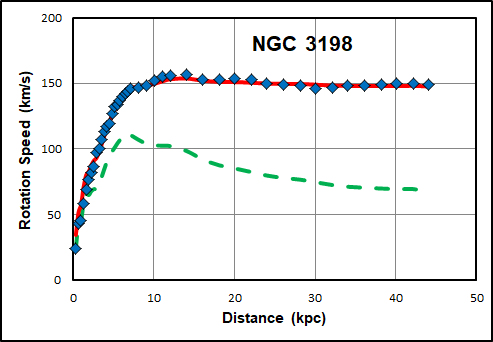
\includegraphics[width=0.8\textwidth]{chapters/c2/figure/ngc3198_sparc}
%  \end{center}
%  \caption{The figure opposite shows the rotation curve for spiral galaxy NGC 3198. The blue diamonds are the observations and reveal the almost flat-like nature of the curve in the outer regions of the galaxy. The dashed green line is the curve for Newtonian gravity. It shows that the rotational velocity should decrease with distance from the galaxy center. The solid red line through the data points is the curve obtained by assuming a simple Gaussian energy scale variation and a simple Gaussian density distribution for the galaxy.}
%  \label{fig:rotation}
%\end{figure}

\par Cosmic Microwave Background (CMB) in Big Bang cosmology, is electromagnetic radiation as a remnant from an early stage of the universe, also known as ``relic radiation''. On the cosmological scale, not only CMB showed evidence of Dark Matter, it also quantifies the amount of Dark Matter in the Universe. Experiments measure the fluctuations of the power spectra of the CMB where Lamda-CDM model are used to  fit the data, which gives the value of the density of baryonic matter, Dark Matter, and Dark Energy.

\par The hot dark matter (HDM) theory\cite{Zeldovich:1982zz} was established in 1980 by Zeldovich's team. The HDM assumes that the light neutrinos made up the majority of the dark matter. It is natural to assume that the dark matter is the weakly coupled particle that already existed in the standard model. However, the conventional neutrino-dominated picture is ruled out by the early universe simulation study in 1983\cite{White:1984yj}. Afterward, scientists realize that only with the slow-paced particle, the so-called ``cold'' dark matter, can prevent the diffusion of small scale fluctuation. As a result, the early universe structure can be formed on all scales, which is consistent with the astronomy observation. Therefore, the cold dark matter theory (CDM theory)\cite{PhysRevLett.48.223} was established in 1983 to explain the cosmic microwave background observation result. Nowadays, as an important part of the standard cosmological model (LambdaCDM theory), the concept of cold dark matter is widely accepted across the astronomers. 

\section{Weakly Interacting Massive Particles}
\par Although the existence of cold dark matter around galaxies and clusters is supported by cosmological observation, scientists still have no clue about what exactly the cold dark matter is. Based on the reductionism, the observation of cold dark matter indicates the existence of weakly interacting fundamental particles. And since the density fluctuation is derived by the cold dark matter candidate mass, and the small scale fluctuation is not supposed to be dissolved, the mass of cold dark matter candidate can not be light. Therefore, the WIMPs - weakly interacting massive particles becomes one of the best candidate particles that characterize the feature of cold dark matter.

\par WIMPs have masses at the electroweak scale from a few GeV to $\mathcal{O}$(TeV), which matchs bserved relic density from CMB analysis.  Both in the two popular beyond SM models Supersymmetry (SUSY) and Extra-dimensions, there are WIMP candidates of DM particles. The electrically neutral lightest supersymmetric particle (LSP) predicted in an R-parity conserved scenario of minimal supersymmetric extension of the Standard Model (MSSM) is an ideal candidates of Dark Matter.  Among all possible choices, the most promising one is the lightest neutralino,which is the lightest state of mixtures of neutral electroweak gauginos and the neutral higgsinos\cite{Feng:2010gw}. Similar to the phenomenology of the MSSM, in minimal universal extra dimensions (MUED) model, each SM particle is accompanied by a partner particle at the first Kaluza-Klein (KK) mode level.

\par Also, the MUED model possesses a geometric parity (KK parity). The lightest partner state (which in MUED is the partner of the $U(1)_Y$ gauge boson) represents dark Matter candidate which matches the observed dark matter relic density\cite{Servant:2002aq}.

\section{Search dark matter in collider experiment}
\par Dark Matter was observed through its gravitational interaction in galaxies. To explore  its further particle properties, several complementary detection methods are used as showed in ~\ref{fig:detection}\cite{Undagoitia:2015gya}: \textbf{direct detection} which aim to observe low-energy recoils (typically a few keVs) of nuclei induced by interactions with particles of dark matter, which (in theory) are passing through the Earth, \textbf{indirect detection} which search for products of the self-annihilation or decay of dark matter particles in outer space, and collider searches looking for WIMPs in Large Hadron Collider (LHC) proton beams. WIMPs particle be detected indirectly as (large amounts of) missing energy and momentum that escape the detectors, provided other (non-negligible) collision products are detected as it should have negligible interactions with normal visible matter. In the following chapters, we will focus on the last method.

%\begin{figure}[htbp]
%  \begin{center}
%    \includegraphics[width=0.5\textwidth]{chapters/c2/figure/DM_detection}
%  \end{center}
%  \caption{Three types of DM particle($\chi$) detection via an interaction with SM particles(P): from right to left the annihilation of DM particles into SM particles (indirect detection), from bottom to top the scattering of DM particles off a nuclei (direct detection), and from left to right the production of DM particles at high energy colliders like the LHC.}
%  \label{fig:detection}
%\end{figure}

\section{Simplified model}
Sample text sample text sample text. Sample text sample text sample text.
Sample text sample text sample text. Sample text sample text sample text.
Sample text sample text sample text. \cite{SimplifiedModels-Alves2012}
